% F2 — ICASSP 2027 manuscript.
% Build with ./build.sh. Numerical assertions are checked by check_numbers.py.
\documentclass[10pt,twocolumn,letterpaper]{article}
\IfFileExists{spconf.sty}{\usepackage{spconf}\newcommand{\usingspconf}{}}{}
\usepackage{amsmath,amssymb,graphicx,booktabs,multirow,url}
\renewcommand{\UrlBreaks}{\do\/\do\-\do\.}
\setlength{\textfloatsep}{3pt plus 2pt minus 2pt}
\setlength{\floatsep}{3pt plus 2pt minus 2pt}
\setlength{\intextsep}{3pt plus 2pt minus 2pt}
\setlength{\abovecaptionskip}{3pt}
\setlength{\belowcaptionskip}{2pt}
\ifdefined\usingspconf\else
  \usepackage[margin=0.75in,columnsep=0.33in]{geometry}
  \newcommand{\name}[1]{\author{#1}}
  \newcommand{\address}[1]{\date{#1}}
  \newcommand{\ninept}{\fontsize{9}{10}\selectfont}
  \newenvironment{keywords}{\par\noindent\textbf{Index Terms---}}{\par}
\fi

\title{Which Conditioning Recording Does a Voice Clone Follow?\\A Balanced Cross-Microphone Crossover}
\name{\shortstack{Rafaello Virgilli\sthanks{Corresponding author: Rafaello Virgilli (rafaello.virgilli@discente.ufg.br).}, Lucas Alc\^antara Souza, Alexandre Costa Ferro Filho, Daniel Tunnermann,\\
Gustavo dos Reis Oliveira, Arlindo Rodrigues Galv\~ao Filho, and Anderson da Silva Soares}}
\address{Advanced Knowledge Center in Immersive Technologies (AKCIT)\\
Federal University of Goi\'as (UFG), Goi\^ania, GO, Brazil}

\begin{document}
\ninept
\maketitle

\begin{abstract}
Voice-clone attribution usually stops at the generator or speaker. We ask a
finer question: which of two same-speaker recording events supplied the
conditioning recording? In a pre-specified complete crossover over 54 VCTK
speakers selected after earlier ECAPA-based screening, we synthesize from each
of two utterances and compare each clone with both utterances recorded through
the other microphone. Four publicly available
cloning systems and four fixed generation texts, distinct from the candidate
transcripts, produce 3,456 clones. Generation uses one
microphone; attribution compares the two events through the other, so speaker
identity, generated text, exact waveform and a shared microphone fingerprint
cannot decide the label. With fixed speaker-verification encoders,
speaker-averaged two-alternative attribution accuracy for
mic1$\rightarrow$mic2 is .896 [.869,.921] for ECAPA and .622
[.593,.652] for WavLM; reversing the microphones gives .907 [.881,.931]
and .620 [.589,.653]. When both candidates are themselves clones from a
different system and a different text, attribution remains .805 [.780,.830]
and .805 [.780,.831] for ECAPA; a replication on a second utterance pair per
speaker, with the decision rule fixed before analysis, gives .906 and .909.
Brackets are 95\% bootstrap intervals that
resample whole speakers within this fixed, previously screened roster;
systems and texts are not resampled. The main evaluation compares two
same-speaker candidates known to include the source event. Attribution remains
high after separate prompt transformations of duration, long-term spectrum and
pitch/energy; these tests do not identify or exclude the carrier, and the
results do not establish whether an arbitrary recording was used.
\end{abstract}

\begin{keywords}
voice cloning, source attribution, audio provenance, speaker verification
\end{keywords}

\section{Introduction}
Zero-shot speech generation conditions on a short reference recording. When
that recording was used without consent, identifying the generator or cloned
speaker does not answer the narrower provenance question: \emph{which recording
was used?} Existing source tracing attributes a synthesis pipeline
\cite{stopa,negroni2026forensic}, and clone attribution identifies an enrolled
speaker \cite{kato2026floor,avatar2026,vcsource2022}. Recording-level evidence
would instead connect an output to one conditioning event among other
recordings of the same voice.

That target is easy to confound. A clone and candidate share speaker identity;
one candidate may be intrinsically closer to every clone; recording session,
duration or microphone can reveal the answer; and generated content may
overlap. Prior prompt-transfer work shows preservation of prosody and acoustic
environment \cite{restyletts2026,noiserobust2024,denoise2025}, while speaker
embeddings themselves encode session and channel \cite{xvecprobe2019,svprobe2026}.
High retrieval from a same-speaker pool therefore does not by itself show that
the target follows the recording used for conditioning.

We turn the question into a balanced intervention. For each speaker, we clone
from recording event A and event B, then test both signed comparisons. Prompt
and candidate are paired captures from different microphones. Four systems and
texts are fully crossed. ECAPA-TDNN \cite{ecapa} (SpeechBrain
\texttt{spkrec-ecapa-voxceleb}) is fixed as the primary encoder, with a
speaker-verification-fine-tuned WavLM \cite{wavlm}
(\texttt{microsoft/wavlm-base-plus-sv}) as a second embedding model for
corroboration. The experiment uses a 54-speaker complement
inherited from ECAPA-informed development rosters. All speakers in that
complement are retained, and metadata alone determines pair selection without
clone outcomes.

We make three contributions. (1) The complete A/B crossover tests whether a
clone follows its conditioning recording after a pickup-path change. (2) The
evaluation, whose analysis plan and decision rule were fixed before outcomes
were inspected, covers 3,456 clones, 54 speakers, four systems and two fixed
representations. (3) The boundary is
explicit: recording-event attribution is consistent in a two-candidate closed
set, but the experiment identifies neither the physical carrier nor deployable
recording-presence detection.

\section{Related work}
\textbf{Attribution and provenance.} Generator tracing, shared-generator
verification and speaker attribution operate above the individual recording
\cite{stopa,negroni2026forensic,kato2026floor,avatar2026}. Recent
source-verification and passive-fingerprint studies distinguish generating
systems and examine attribution cues \cite{falez2025,negroni2025source,li2026fingerprints};
our label instead identifies the conditioning event within one speaker.
Watermarking requires
instrumentation before misuse \cite{vocalock}; VoiceMark attributes cloned
speech through a watermark embedded in its inference-time reference
\cite{voicemark}, whereas our candidates are unmodified recordings. Training-set
membership inference asks whether audio entered training \cite{flowleak2026}, and VoxGuard
tests enrolled-speaker and attribute privacy \cite{voxguard2026}; neither asks
which recording was the inference-time prompt. We found no prior controlled study that intervenes on
the prompt recording within speaker while changing the candidate pickup path.

\textbf{Prompt transfer and nuisance information.} Training-free generator
attribution uses frozen representations \cite{tada2025,pirlogeanu2026}, and
recording-related nuisance in speaker embeddings motivates cross-recording
sampling \cite{ssps2025}. Prompt-conditioned systems transfer prosody and
environment \cite{restyletts2026,noiserobust2024,icl2026}, although cloning
also alters style systematically \cite{stylecloning2026}; prompt cosine is a
standard synthesis metric \cite{simo}. Exact prosody
cloning transfers reference prosody \cite{prosodyclone2022}. Source-voiceprint
tracing recovers identity from converted audio \cite{sourcevoiceprint2023},
while rank/local-disclosure work treats linkage without global thresholds
\cite{rankdisclosure2026,sterns2026}. None intervenes on which of two
same-speaker recording events conditions a clone. Concurrent work separates
prompt environment from identity \cite{promptenv2026}. These works motivate
recording-level leakage but do not identify the chosen event. We target
\emph{A versus B}, not generic clone--prompt resemblance.

\section{Cross-microphone crossover}
\subsection{Task and design}
For speaker $s$, let recording events $A$ and $B$ each have paired VCTK
mic1/mic2 captures \cite{vctk}: a DPA 4035 omni and a Sennheiser MKH 800.
That the two are genuinely distinct signals is the design's load-bearing
assumption. We tested it rather than assuming it. Raw correlation cannot settle
the question. A delayed copy can score near zero, while genuine pairs reach $.92$ median
once delay-aligned. We therefore use the normalized least-squares residual
$\min_{g,|\tau|\le 50\,\mathrm{ms}}\|y-g\,T_\tau x\|_2/\|y\|_2$ over a scalar
gain $g$ and a zero-padded delay $T_\tau$, where $x$ and $y$ are the mic1 and
mic2 captures; its $.00001$ duplicate bar
is a numerical tolerance for these transforms, not a universal perceptual
threshold. Across all 108 event captures, the residual is $.38$ median
(range $.21$--$.70$). Exact, gain-scaled and delayed injections on every source,
including both delay-window boundaries, are at most $.000000026$; no pair is byte-identical. A clone $c_{A,m1}$ is conditioned on
event A's mic1 capture.
The primary comparison asks whether a fixed encoder $f$ gives
\begin{equation}
  I\!\left[\cos(f(c_{A,m1}),f(A_{m2}))>
              \cos(f(c_{A,m1}),f(B_{m2}))\right],
\end{equation}
with ties worth $1/2$. We also clone from B and reverse the correct label. Thus
an encoder's unconditional preference for A cannot create a positive effect.
The predeclared direction reversal swaps microphones (mic2 prompt, mic1 candidates)
and cannot rescue a failed primary direction.

With $q(u,v)=\cos(f(u),f(v))$ and $d_X=q(c_X,A)-q(c_X,B)$ on
opposite-microphone candidates, a cell contributes
$\{I[d_A>0]+I[d_B<0]\}/2$. Clone-independent candidate bias therefore yields
chance; ties receive $1/2$.

The threat model is deliberately narrow. The analyst has a clone and two
same-speaker candidate recordings; exactly one is the other-microphone capture
of the event that supplied the conditioning recording.
The objective is source attribution, not deciding whether an arbitrary
recording was used. Encoder parameters, score direction and the tie rule are
fixed before evaluation. The analyst does not train on these speakers or
systems.

\begin{figure}[t]
\centering
\fbox{\parbox{.94\linewidth}{\centering
\textbf{Primary: opposite-pickup attribution}\\[-1pt]
$A_{m1}\!\rightarrow\!c_{A,m1}\!\rightarrow\!\{A_{m2},B_{m2}\}$\quad and\quad
$B_{m1}\!\rightarrow\!c_{B,m1}\!\rightarrow\!\{A_{m2},B_{m2}\}$\\[-1pt]
Correct labels are reversed across arms; speaker, system and generated text are
held fixed. The direction-reversal analysis swaps $m1$ and $m2$.}}
\caption{Complete two-arm crossover. Generation never consumes the microphone
used for the attribution candidates.}
\label{fig:design}
\end{figure}

\begin{table}[t]
\centering
\caption{What the crossover blocks, and the residual scientific boundary.}
\label{tab:controls}
\resizebox{\linewidth}{!}{%
\begin{tabular}{lll}
\toprule
Shortcut & Design response & Residual \\
\midrule
Speaker identity & A/B within speaker & none for the label \\
Candidate preference & both signed arms & arm interactions \\
Generated content & four texts shared A/B & text fixed, not sampled \\
Exact waveform/device & opposite microphone & event acoustics \\
Duration/text length & metadata-matched A/B & other local cues \\
\bottomrule
\end{tabular}}
\end{table}

\subsection{Frozen roster and generation}
VCTK v0.92 documents DPA 4035 and Sennheiser MKH 800 microphones in a fixed
hemi-anechoic setup \cite{vctk}. Its public description does not establish
acquisition timing, so our claim requires paired captures, not simultaneity.
The frozen manifest independently supports the pairing: all 108 selected
event/microphone pairs have identical frame counts and sampling rates.

The 54-speaker roster is the exact complement of two earlier development
subsets. The first applied an ECAPA pair-separation screen to 105 speakers
(pair cosine below that speaker's 90th percentile over pairs of
duration-eligible utterances) and retained the lexicographically first 30
passing speakers. The second retained all 24 remaining speakers with one
eligible pair at ECAPA cosine distance $\leq.20$ and another at $\geq.38$,
pair-mean durations within .50\,s. The roster is therefore disjoint from those
two subsets, although its speakers appeared in an earlier exploratory screen.
It is blind to this experiment's clone outcomes, but not embedding-naive or
population-sampled. Within that fixed complement, all 54
speakers remain. The A/B-pair rule below never inspects an embedding, score or clone outcome.

For each speaker, selection enumerates 4--10\,s paired utterances and excludes
the conditioning utterance used for that speaker in the earlier exploratory
screen (listed in the public selection manifest). It requires an A/B duration
gap of at most .25\,s and a relative seconds-per-UTF-8-byte gap
$|r_A-r_B|/[(r_A+r_B)/2]$ of at most 5\% on \emph{both} microphones. A
deterministic metadata-only rule then takes the lexicographic minimum of the
largest tolerance-normalized gap, their sum, the largest rate gap and the
largest duration gap; no embedding, score or clone outcome enters within-roster
pair selection.
Transcripts A and B differ. Generation instead uses four fixed texts that are
disjoint from both candidates and fully crossed across arms. These four texts
were also used in our earlier experiments; they are fixed experimental factors.
A post-hoc ASR screen (Whisper-large-v3-turbo) gives median WER .04 against
the requested text; no clone (0 of 3,456) was flagged for four or more
consecutive recognized words shared with its conditioning transcript after
excluding sequences present in the requested text. This diagnostic does not
establish the absence of reference-speech repetition. The selected
roster is substantially tighter than the eligibility limits. Its worst duration gap is .112\,s,
and its worst relative duration-per-byte gap is 2.57\% across either microphone.

We evaluate F5-TTS (f5-tts 1.1.22) \cite{f5tts}, XTTS-v2 (coqui-tts 0.25.3)
\cite{xtts}, CosyVoice~2 \cite{cosyvoice2} and Seed-VC \cite{seedvc}; exact
checkpoint revisions are listed in the public artifact. Seed-VC converts one
fixed LibriTTS-R \cite{librittsr} source utterance per generation text, shared
across targets. The full design is
$54$ speakers $\times2$ events $\times2$ prompt microphones $\times4$ texts
$\times4$ systems $=3{,}456$ clones. Exact checkpoints, repositories,
environments, files and per-clone ancestry ledgers are hash-pinned.

\subsection{Estimand and decision criteria}
Each speaker contributes 32 dependent comparisons per direction (two arms,
four systems, four texts). We first average within speaker, then give all 54
speakers equal weight. Percentile intervals resample whole speaker vectors
100,000 times with a frozen seed. They quantify stability to speaker
composition in this fixed eligible roster, not population-coverage confidence.
Systems and texts are fixed crossed factors; system-specific points are
descriptive and receive no individual inferential claims.

The primary success criteria, fixed before outcomes were inspected, were ECAPA
accuracy $\geq.80$ with lower stability-interval endpoint $>.70$, and WavLM
lower endpoint $>.50$; the .80/.70 rule is an author-declared large-effect
criterion, not a deployment-utility claim. Both reversed-microphone estimates
are reported; we claim corroboration after reversal only if both lower
endpoints exceed .50. Diagnostics cannot
rescue any criterion.

We fixed the roster, analysis settings and success criteria before inspecting
outcomes. A second, independent
recomputation rehashed 3,456 clones and ledgers plus 216 candidates and
reproduced every result field to $2\times10^{-15}$. The released artifact
contains per-clone cosine scores with candidate identities and an independent
verifier that reconstructs the 3,456-row identity
grid, bootstrap and verdict without audio or model weights.

\section{Results}
\subsection{The conditioning event survives pickup change}
Table~\ref{tab:pooled} reports the predeclared directions. ECAPA attributes the
conditioning event in 89.6\% of primary comparisons and 90.7\% in reverse. It
therefore meets the .80/.70 primary bar. WavLM is much weaker but directionally
consistent at 62.2\%/62.0\%. All five predeclared criteria pass: the four
lower endpoints in Table~\ref{tab:pooled} (.869, .593, .881, .589) exceed .50,
the primary ECAPA point .896 reaches .80 and its lower endpoint .869 exceeds
.70. The ECAPA effect meets the frozen large-effect rule, and WavLM
corroborates its direction.

\textbf{Clone candidates.} A stricter comparison, whose grid and decision rule
were fixed before analysis, replaces both real candidates by clones: the query
clone is compared with two clones of the same speaker made by a different
system from a different text, conditioned on events A and B through the
opposite microphone (288 comparisons per speaker and direction). The correct
candidate shares only the conditioning event. Attribution remains .805
[.780,.830] and .805 [.780,.831] for ECAPA and .610 [.595,.626] and .612
[.593,.632] for WavLM (Table~\ref{tab:pooled}, Clone-to-clone column), so the event
information survives a change of generator, output text, microphone and
candidate medium.

\textbf{Fresh pairs.} A replication with the decision rule fixed before
analysis re-runs the crossover on a second utterance pair per speaker, chosen
by the same metadata-only rule after excluding the original pair (53 speakers;
one admits no second pair; 3,392 clones). The rule passes again: ECAPA .906
[.878,.931] and .909 [.883,.933], WavLM .666 and .644
(Table~\ref{tab:pooled}). Observed per-speaker ECAPA accuracies have Pearson
correlations .061/.291 between the two utterance pairs; this descriptive
comparison does not establish the stability of an underlying speaker effect.

\begin{table}[t]
\centering
\caption{Speaker-averaged two-alternative attribution accuracy [95\%
speaker-resampling stability interval]; 1,728 comparisons per direction
(clone-to-clone: 15,552; fresh pairs: 53 speakers, 1,696). Clone-to-clone
candidates come from a different system and text; fresh pairs are a second,
disjoint utterance pair per speaker.}
\label{tab:pooled}
\resizebox{\linewidth}{!}{%
\begin{tabular}{llccc}
\toprule
Prompt$\rightarrow$candidate & Encoder & Cross-mic & Clone-to-clone & Fresh pairs \\
\midrule
mic1$\rightarrow$mic2 & ECAPA & \textbf{.896 [.869,.921]} & .805 [.780,.830] & .906 [.878,.931] \\
                      & WavLM & \textbf{.622 [.593,.652]} & .610 [.595,.626] & .666 [.636,.696] \\
mic2$\rightarrow$mic1 & ECAPA & \textbf{.907 [.881,.931]} & .805 [.780,.831] & .909 [.883,.933] \\
                      & WavLM & \textbf{.620 [.589,.653]} & .612 [.593,.632] & .644 [.616,.673] \\
\bottomrule
\end{tabular}}
\end{table}

\begin{figure}[t]
\centering
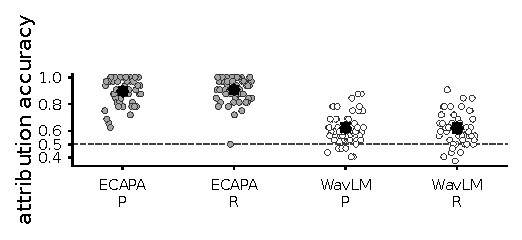
\includegraphics[width=.90\linewidth]{fig_exp205_speakers.pdf}
\caption{Fixed-roster speaker means (54 dots/group; 32 comparisons per dot).
Diamonds and bars are pooled points and 95\% speaker-resampling stability intervals;
the dashed line is chance. P/R: primary/reverse.}
\label{fig:speakers}
\end{figure}

Same-microphone diagnostics, never verdict inputs, are only modestly higher
(ECAPA .938/.930, WavLM .631/.659, primary/reverse): exact pickup identity is
unnecessary, though paired captures of one event do not establish microphone
invariance.

Figure~\ref{fig:speakers} exposes the heterogeneity hidden by pooled points.
All 54 primary ECAPA speaker means exceed .50; in reverse, 53 exceed it and one
equals it. WavLM is not uniformly positive: 47 primary and 43 reverse speaker
means exceed .50, so its role is aggregate corroboration, not a per-speaker
guarantee. Whole-speaker resampling preserves this heterogeneity rather than
treating 1,728 comparisons per direction as independent.

\subsection{Breadth across fixed systems}
Table~\ref{tab:systems} gives descriptive system points. ECAPA exceeds .82
throughout, while WavLM spans .572--.671 and has weaker XTTS-v2 cells. The
systems are fixed, and there are no simultaneous per-system intervals. The
breadth claim is therefore limited to this tested design.

\begin{table}[t]
\centering
\caption{Descriptive attribution-accuracy points by system. P/R: primary/reverse.}
\label{tab:systems}
\resizebox{\linewidth}{!}{%
\begin{tabular}{lcccc}
\toprule
Encoder, dir. & F5-TTS & XTTS-v2 & CosyVoice~2 & Seed-VC \\
\midrule
ECAPA, P & .942 & .833 & .910 & .898 \\
ECAPA, R & .942 & .822 & .942 & .924 \\
WavLM, P & .618 & .572 & .671 & .627 \\
WavLM, R & .657 & .574 & .657 & .593 \\
\bottomrule
\end{tabular}}
\end{table}

The ECAPA--WavLM gap rules out near-ceiling magnitude for every representation;
WavLM's positive lower endpoints still oppose ECAPA-weight specificity. Both are
speaker-verification embeddings, so a shared cue remains possible. Mean
correct-minus-incorrect cosine margins are positive but small, ECAPA .079/.081
and WavLM .011/.013 for primary/reverse, and are descriptive only.

\subsection{Descriptive sensitivity analyses}
Table~\ref{tab:ancestry} stratifies the inherited ECAPA-informed complement by
the earlier pair-separation screen. Direction persists among 36 pass-but-not-retained and
15 fail speakers; three absent from that record remain separate. This post-hoc
check cannot create an embedding-naive sample or alter the pooled verdict.

Only the crossover, the clone-candidate comparison and the fresh-pair
replication have decision rules fixed before analysis; the remaining analyses
are post-hoc and descriptive. Two such
extensions bound the claim. Enlarging the candidate set with
metadata-matched captures of the same speaker through the opposite microphone,
among the 22 speakers with enough eligible captures, ECAPA rank-1 accuracy
decreases from .935/.913 with two candidates to .635 [.545,.720]/.587
[.510,.659] with sixteen (704 comparisons per direction; sixteen-candidate
chance .0625). Re-synthesizing each primary-direction clone with a
different system and a different text, the second-generation clone is still
attributed to the original event at .796 [.759,.832] (ECAPA) and .596
[.568,.626] (WavLM).

\begin{table}[t]
\centering
\caption{Post-hoc points by status in the earlier pair-separation screen. P/R:
microphone direction; no stratum-specific claim.}
\label{tab:ancestry}
\resizebox{\linewidth}{!}{%
\begin{tabular}{lccc}
\toprule
Screen status & $n$ & ECAPA P/R & WavLM P/R \\
\midrule
Pass, not retained & 36 & .908/.907 & .609/.596 \\
Fail                & 15 & .879/.915 & .654/.685 \\
Not evaluated       &  3 & .833/.875 & .625/.583 \\
\bottomrule
\end{tabular}}
\end{table}

Arm-separated points also oppose a one-candidate shortcut. For A/B, ECAPA is
.889/.903 in primary and .892/.922 in reverse; WavLM is .588/.656 and
.660/.581, respectively. Thus WavLM's arm asymmetry reverses with microphone
direction. Descriptively, all 32
system$\times$direction$\times$encoder$\times$arm cells are above .50 (minimum .523).
No cell has a separate interval or multiplicity-adjusted test.

\subsection{What changed relative to earlier evidence}
An earlier exploratory two-reference crossover (30 speakers, 960 trials)
obtained .806 [.757,.854] on one pickup path with favorable reference pairs
and missed its frozen .90 point bar; we retain it as positive discovery, not
confirmation. The present experiment is a separate test (54-speaker complement,
all speakers retained, metadata-only A/B pairs, balanced labels,
opposite-microphone candidates, fixed readouts) with its own frozen .80/.70
ECAPA bar; passing it does not retroactively change the earlier .90 miss.

\section{Boundary and limitations}
\textbf{Attribution is not presence detection.} The crossover is a closed-set
two-alternative question known to contain the source. Table~\ref{tab:presence}
sweeps one common threshold per encoder over the same scores, pooled over
systems and arms, as one-to-one verification within speaker. At the .01 prior,
minimum DCF sits at or near the reject-all cost of 1.000; whole-speaker
resampling as in Table~\ref{tab:pooled} gives ECAPA upper endpoints .989/.989.
At the .5 prior of the two-candidate threat model it is .67/.68 and .88/.89. This
post-hoc check is descriptive. A score can order A above B while no global
threshold separates the two.

\begin{table}[t]
\centering
\caption{Within-speaker one-to-one verification with one global threshold:
EER and normalized minimum DCF. Target: clone versus its own event;
non-target: clone versus the same speaker's other event; 1,728 each per
direction. $C_{miss}=C_{fa}=1$.}
\label{tab:presence}
\resizebox{\linewidth}{!}{%
\begin{tabular}{llccc}
\toprule
Encoder & Prompt$\rightarrow$candidate & EER (fraction) & minDCF, prior .01 & minDCF, prior .5 \\
\midrule
ECAPA & mic1$\rightarrow$mic2 & .337 & .980 & .667 \\
ECAPA & mic2$\rightarrow$mic1 & .343 & .981 & .678 \\
WavLM & mic1$\rightarrow$mic2 & .447 & 1.000 & .884 \\
WavLM & mic2$\rightarrow$mic1 & .451 & .998 & .889 \\
\bottomrule
\end{tabular}}
\end{table}
We therefore restrict investigative triage to a known-positive two-recording set
for human provenance review, where the score can prioritize candidates. It
cannot decide whether an arbitrary queried recording was present, and it is not
an automated accusation.

\textbf{The carrier is unidentified.} Opposite microphones exclude an exact
waveform and shared device fingerprint, while A/B balancing excludes a fixed
candidate preference, and metadata matching sharply limits duration shortcuts.
Three separate post-hoc prompt transformations, synthesized with the same
systems and scored against unmodified candidates (primary direction), test
robustness rather than mechanism: ECAPA accuracy was .896 after
total-duration equalization, .893 after smoothed long-term spectral
equalization and .840 [.804,.874] after pitch/energy modification (.866 when
the candidates receive the same transform), against .896 for the original
prompts. These transformations do not isolate causal contributions: relative
timing and residual spectral information may remain, and the pitch/energy
comparison includes resynthesis effects. Post-hoc alternative readouts on the
same grid remain below ECAPA: a long-term spectral and cepstral average reaches
.548/.549, and mean-pooled WavLM layer 0, centred on the speaker's real-capture
mean, reaches .633/.631 against .622/.620 for WavLM-SV. The carrier therefore
stays bundled in event-level prosody, articulation, background acoustics,
paired-capture room state and their interactions with model conditioning.

\textbf{Scope.} The result concerns four fixed checkpoints, four fixed texts,
read English speech and one inherited 54-speaker VCTK complement. The complement
is disjoint from the earlier development rosters but ECAPA-informed through
their composition, not globally unseen or population-sampled. Checkpoint
training corpora are not documented at recording level, so VCTK exposure cannot be
excluded. The intervals do not sample systems, texts or a speaker
population. Spontaneous conversational speech, noisy field recordings, other
pickup paths, candidate sets beyond sixteen and open-set search remain
untested; larger candidate sets were examined only post hoc on eligible
subsets.

\textbf{Release and misuse.} Code, score-level data, provenance metadata and
aggregate/per-speaker results are at \url{https://github.com/rvirgilli/voice-clone-cross-microphone-crossover/tree/f2-icassp2027-rc2};
model weights, source audio and
playable impersonations are not redistributed.
Recording attribution can assist provenance audits, but it can also deanonymize
speakers; licensing alone does not settle consent.

\section{Conclusion}
In this fixed roster, clones preferentially match the other-microphone capture
of their conditioning event across the two tested microphone paths. ECAPA meets the frozen large-effect
criterion, and WavLM shows a smaller effect in the same direction. That
direction persists when the microphone roles are reversed, when both
candidates are clones from another system and text (.805), on a second
utterance pair per speaker (.906/.909), and after a second synthesis (.796). The primary and
reverse pooled estimates weight the four fixed systems equally. This is a large closed-set signal between two
tested microphone paths; its physical carrier remains unidentified, and the
experiment does not solve open-set recording-presence detection.

\let\oldthebibliography\thebibliography
\renewcommand{\thebibliography}[1]{\oldthebibliography{#1}%
  \setlength{\itemsep}{0pt}\setlength{\parsep}{0pt}\setlength{\topsep}{2pt}}
{\small
\bibliographystyle{IEEEbib}
\bibliography{refs}
}
\end{document}
